\chapter{Android 集成环境及相关技术}
\section{Android 起源与发展}
Android(安卓)是一种以 Linux 为基础的开放源码操作系统。 Android 操作系统
最初由 Andy Rubin 开发,主要支持手机,2005 年由 Google 收购注资,并拉拢多家制
造商组成开放手机联盟开发改良,逐渐扩展到平板电脑及其他领域上。Google 在 2007
年正式推出该系统后,在短短的几年时间内得到了广泛的应用。截至 2011 年 9 月份,
Android 系统的应用数目已经达到了 48 万,而在智能手机市场,Android 系统的占有率
已经达到了 43\%,并在亚太地区市场占据统治地位,终结了 Symbian(塞班系统)的霸
主地位,跃居全球第一。2012 年 7 月美国科技博客网站 Business Insider 评选出二十一
世纪十款最重要电子产品,Android 操作系统榜上有名。目前 Android 系统主要使用于
便携设备,广泛应用于智能手机、平板电脑、MID 等电器。截止目前,Android 最新版
本号为 2013 年 11 月 01 日正式发布的 Android 4.4 KitKat(奇巧巧克力)。

\section{Android 平台特性与架构}
\subsection{Android 平台的特性}
Android 平台采用了整合的策略思想,包括底层 Linux 操作系统、中间层的中间件
和上层的 Java 应用程序。其基本特性如下\cite{4}:

(1) 应用程序框架支持组件的重用与替换。支持用户根据自己的喜好自定义自己
的手机系统应用程序。

(2) Dalvik 虚拟机专门为移动设备进行了优化。Android 应用程序将由 Java 编写、
编译的类文件通过 DX 工具转换成一种后缀名为.dex 的文件来执行。Dalvik 虚拟机是基
于寄存器的,相对于 Java 虚拟机速度要快很多。

(3) 内部集成浏览器基于开源的 WebKit 引擎。内置的浏览器,宣告了真正的移
动互联网时代的来临,手机就是一台“小电脑”,可以满足用户随时随地的上网需求。

(4) 优化的图形库包括 2D 和 3D 图形库,其中 3D 图形库基于 OpenGL ES 1.0。
强大的图形库给游戏开发带来福音,同时也极大的提高了用户体验。

(5) SQLite 用作结构化的数据存储。

(6) 对多媒体支持,包括常见的音频、视频和静态印象文件格式,如 MPEG4、
H.264、MP3、AAC、AMR、JGP、PNG、GIF 等。

(7) GSM 电话(依赖于硬件)。

(8) 蓝牙(Bluetooth)、EDGE、3G、WiFi(依赖于硬件)。

(9) 照相机、GPS、指南针和加速度计(依赖于硬件)。

(10) 丰富的开发环境包括设备模拟器、调试工具、内存及性能分析图表和 Eclipse
集成的开发环境插件。Google 提供了 Android 开发包 SDK,其中包含了大量的类库和开
发工具,并且针对 Eclipse 的可视化开发插件 ADT。

基于其以上特性,Android 操作系统相比 iPhone、Windows Phone 等系统有以下优
势\cite{5}:

(1) 彻底的开放性与免费性。Android 是一个对第三方软件完全开放的平台,开
发者在为其开发程序时拥有更大的自由度,允许任何移动终端厂商加入到 Android 联盟
中。

(2) 挣脱运营商的束缚。Android 的出现使用户可以更加方便地连接网络,随着
EDGE、HSDPA 这些 2G 至 3G 移动网络的逐步过渡和提升,手机应用对运营商的依赖
与局限进一步降低。

(3) 丰富的硬件选择。得益于 Android 的开放性,众多的厂商会推出丰富多彩、
各具特色的多种产品。功能上的差异和特色却不会影响到数据同步、甚至软件的兼容性。

(4) 不受任何限制的开发商。Android 平台提供给第三方开发商一个十分宽泛自
由的环境,因此不会受到各种条条框框的阻挠,这促使了众多新颖别致的软件的诞生。

(5) 无缝结合的 Google 应用。Android 作为在互联网领域已经走过十多年历史、
从搜索巨人到互联网应用等各方面均有所渗透的网络巨擘 Google 推出的智能手机系统,
Android 手机将无缝结合诸如 Google 地图、邮件、搜索等服务应用。

\subsection{Android 平台的架构}
\begin{figure}[htbp]
    \centering
    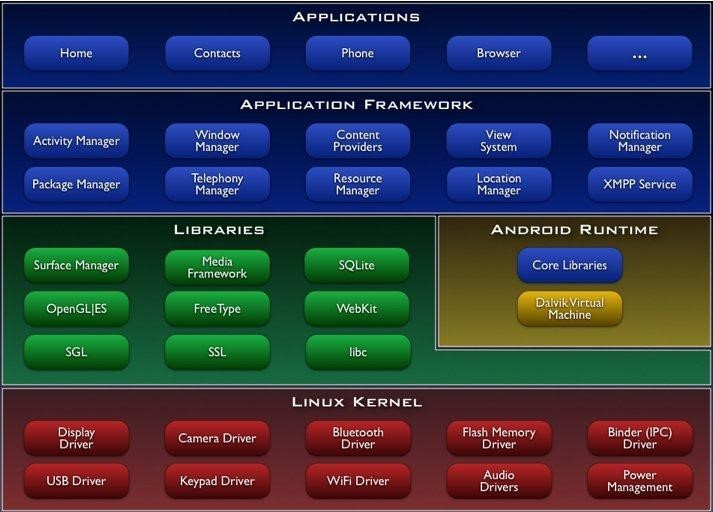
\includegraphics[width=0.9\linewidth]{201}
    \caption{\label{fig:201}Android 操作系统的体系结构}
\end{figure}

如\autoref{fig:201}所示,Android 操作系统的体系结构可分为 4 层,由上到下依次是应用程
序、应用程序框架、核心类库和 Linux 内核,其中第三层还包括 Android 运行时的环境。

(1) 程序应用。Android 连同一个 Java 编写的核心应用程序包一起发布,该应用
程序包包括常见的应用有 E-mail 客户端、SMS 短消息接法程序、行程日历、地图导航、
网络浏览器、通讯录管理程序等。

(2) 应用程序框架。开发者完全可以访问核心应用程序所使用的 API 框架。该应
用程序框架架构用来简化组件软件的重用,任何一个应用程序在遵循框架的安全性限制
的条件下都可以发布它的功能块并且任何其他的应用程序都可以使用其所发布的功能
块。该应用程序重用机制使得组件可以被用户替换。以下所有的应用程序都由一系列的
服务和系统组成,包括:可扩展的视图(Views)、内容管理器(Content Providers)、
资源管理器(Resource Manager)、通知管理器(Notification Manager)、活动类管理器
(Activity Manager)等。

(3) Android 程序库。Android 包括一个被 Android 系统中各种不同组件所使用的
C/C++集库。该库通过 Android 应用程序框架为开发者提供服务。其主要的核心库包括
为基于 Embedded Linux 的设备定制的系统 C 库、支持多种媒体资源的媒体库、为多个
应用程序提供 2D 和 3D 图层的无缝融合的 Surface Manager、LibWebCore 、内置的 2D
图形引擎 SGL、可以使用硬件 3D 加速的 3D libraries、用于位图(bitmap)和向量(vector)
字体显示的 FreeType、轻型关系型数据库引擎 SQLite 等。

(4) Android 运行库。Android 包括了一个提供了 Java 编程语言核心库的大多数
功能核心库。每一个 Android 应用程序都在它自己的进程中运行,都拥有一个独立的
Dalvik 虚拟机实例。Dalvik 虚拟机依赖于 Linux 的线程机制和底层内存管理机制等功能,
基于寄存器的,所有的类都是经由 Java 汇编器编译,然后通过 SDK 中的 DX 工具转化
成.dex 格式由虚拟机执行。

(5) Linux 内核。Android 的核心系统服务依赖于 Linux 内核,如安全性、内存管
理、进程管理、网络协议栈和驱动模型。Linux 内核也同时作为硬件和软件栈之间的硬
件抽象层。

\section{Android 平台应用程序组件及其工作机制}
Android 的一个特点是:在一个应用允许的情况下,其他应用程序可以使用这个应
用的元素。构成一个独立的 Android 应用程序的组件共有四类,分别是 Activity、Service、
Content Provider、Broadcast Receiver\cite{6}。

(1) Activity。Activity 是 Android 构造块中最基本的一种,一个 Activity 通常展
现为一个可视化的用户界面,是 Android 程序与用户交互的窗口,也是 Android 组件中
最基本也是最复杂的一个组件。从视觉效果来看,一个 Activity 占据当前的窗口,响应
所有窗口事件,具备有控件,菜单等界面元素。从内部逻辑来看,Activity 需要为了保
持各个界面状态,需要做很多持久化的事情,还需要妥善管理生命周期,和一些转跳逻
辑。对于开发者而言,需要派生一个 Activity 的子类,进而进行编码实现各种功能方法。
而 Activity 之间需要通过 Intent 进行通信。

(2) Service。Service 通常位于后台运行,它一般不需要与用户交互,因此 Service
组件没有图形用户界面。Service 组件需要继承 Service 基类。Service 组件通常用于为其
他组件提供后台服务或监控其他组件的运行状态。其与 Activity 在 Android 的概念方面
比较接近,均需封装有一个完整的功能逻辑实现,接受上层指令,完成相关的事件,定
义好需要接受的 Intent 提供同步和异步的接口。Service 执行长时间运行的操作,或运程
进程执行工作,且不会阻塞用于与其他 Activity 的交互。

(3) Content Provider。作为应用程序之间唯一的共享数据的途径,Content Provider
主要的功能就是存储并检索数据以及向其他应用程序提供访问数据的接口。在 Android
系统中,每个应用程序都是用自己的用户 ID 并在自己的进程中运行,每个进程都拥有
独立的进程地址空间和虚拟空间。这样可以有效地保护系统及应用程序,避免被其他不
正常应用程序所影响。Android 的数据(包括 files, database 等)都是属于应用程序自
身,其他的应用是不能访问到的,更无法直接进行操作。为了使其他程序能够操作数据,
可以通过做成 Content Provider 组件提供数据操作的接口。Android 提供了一些主要数据
类型的 Content provider,比如音频、视频、图片和私人通讯录等。可在 android.provider
包下面找到一些 android 提供的 Content provider。

(4) Broadcast Receiver。Broadcast Receiver 不参与执行任何任务。广播是一种广
泛运用的在应用程序之间传输信息的机制。而 Broadcast Receiver 是对发送出来的广播
进行过滤接收并响应的一类组件。Broadcast Receiver 不包含任何用户界面。然而它们
可以启动一个 Activity 或者 Service 以响应接受到的信息,或者通过 Notification Manager
通知用户。Broadcast Receiver 通知用户有新的通知产生的方式还包括:闪动背景灯、震
动设备、发出声音等等。通常程序会在状态栏上放置一个持久的图标,用户可以打开这
个图标并读取通知信息。

\section{Android 平台应用开发环境}
\begin{figure}[htbp]
    \centering
    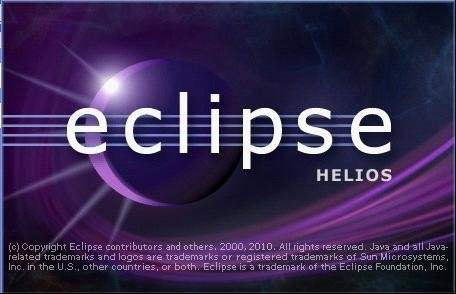
\includegraphics[width=.7\linewidth]{202}
    \caption{\label{fig:202}Eclipse 启动界面}
\end{figure}
如\autoref{fig:202},Eclipse 是一个开放源代码的、基于 Java 的可扩展开发平台。就其本身而
言,它只是一个框架和一组服务,用于通过插件组件构建开发环境。Eclipse 附带了一
个标准的插件集,包括 Java 开发工具(Java Development Kit,JDK)。在本文的研究与
开发中选择了 Windows7 系统下的 Eclipse 软件作为开发环境。其开发环境搭建步骤可分
为以下几个步骤\cite{7}。

(1)Java 环境的搭建

在 Java 官网上选择同意协议之后选择适合的 JDK(Java Development kit,即 Java
开发套件)版本下载,选定安装路径安装完成后需配置系统环境变量,在新建的 CMD
窗口下分别输入“java -version”与“javac”命令,若得到如\autoref{fig:203}的显示结果,则此步搭
建完成。

\begin{figure}[htbp]
    \centering
    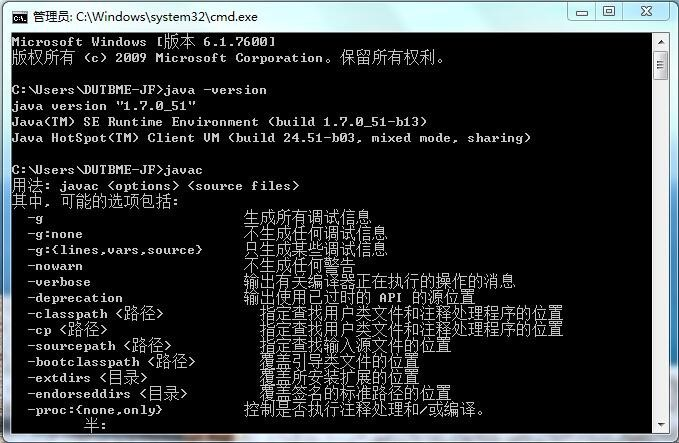
\includegraphics[width=.8\linewidth]{203}
    \caption{\label{fig:203}测试 Java 环境是否搭建完成}
\end{figure}

(2)安装 Android SDK

在官网上下载 Android SDK,默认方式安装即可。安装成功之后自动打开 Android
SDK Manager 更新相关 packages 即可,如\autoref{fig:204}所示。

\newpage

\begin{figure}[htbp]
    \centering
    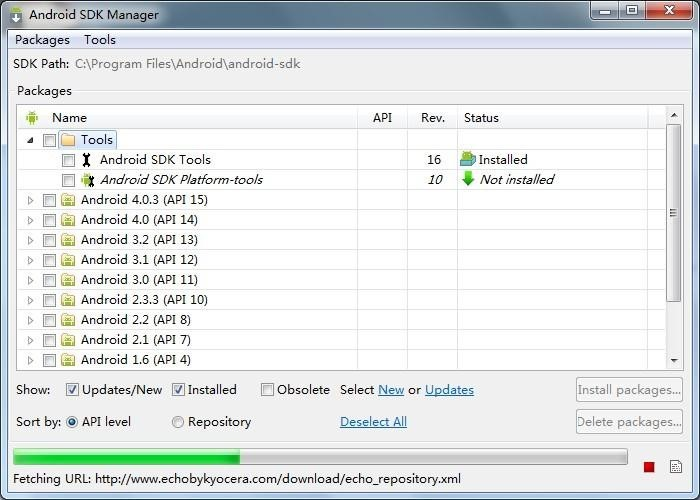
\includegraphics[width=.65\linewidth]{204}
    \caption{\label{fig:204}更新 packages}
\end{figure}

% \vspace{-10pt}
(3)安装并配置 Eclipse

将下载的 eclipse-jee-indigo-SR1-win32.zip 解压缩至任一路径,打开 eclipse.exe,启
动 Eclipse,设置 WorkSpace 之后,点击 Help->Install New Software。点击“Add”,弹
出对话框,在 Location 栏输入:http://dl-ssl.google.com/android/eclipse。按照提示说明,
选择同意协议进行相关软件的安装。

\begin{figure}[htbp]
    \centering
    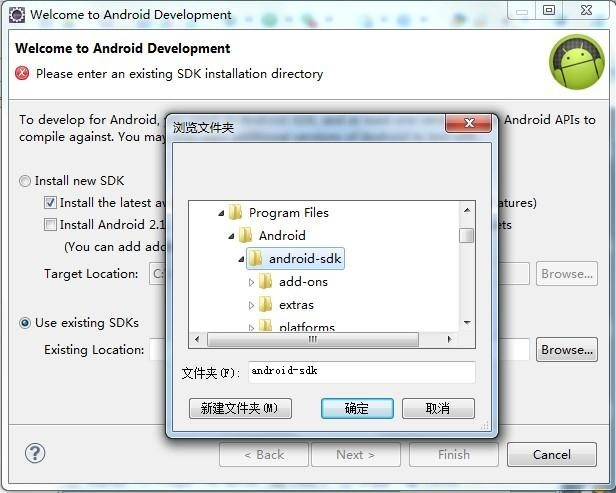
\includegraphics[width=.65\linewidth]{205}
    \caption{\label{fig:205}选择 SDK 安装路径}
\end{figure}

安装完毕重启 Eclipse 后点击 Windows->Preferences->Android->Browse,选择 SDK
Location 为前述 SDK 安装路径,如\autoref{fig:205}所示。选择路径后重新打开上述页面,若出现
\autoref{fig:206}所示的结果,则此步搭建工作完成。

\begin{figure}[htbp]
    \centering
    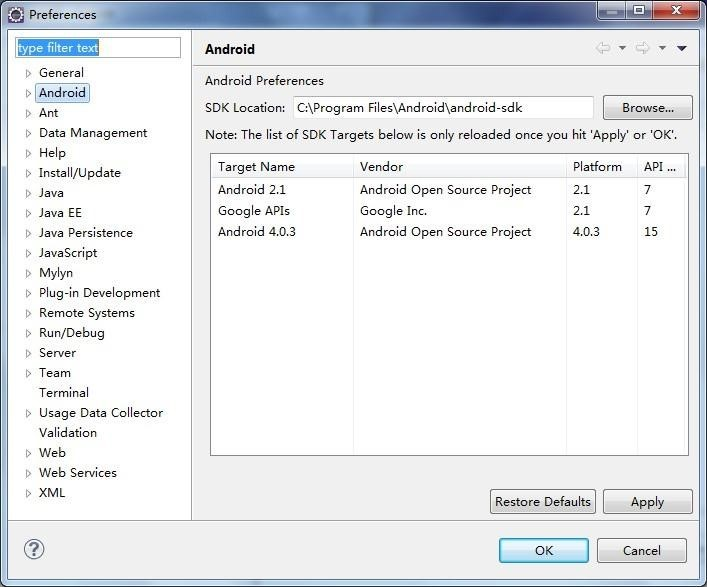
\includegraphics[width=.7\linewidth]{206}
    \caption{\label{fig:206}配置完成的信息界面}
\end{figure}

\section{本章小结}
本章比较全面的介绍了 Android 操作系统平台以及在此平台上编程的相关知识,详
细分析了 Android 的特点与优势,对其硬件架构原理进行了说明,重点介绍了其四大组
件的工作机制。最后完整介绍了 Android 平台应用开发环境的搭建过程。本章旨在为第
四章、第五章的心电处理分析系统的编程奠定相应的基础。